\documentclass{article}
\usepackage{amsmath}
\usepackage{tikz}
\usetikzlibrary{arrows.meta}

\begin{document}

The graph \( E_{(m_1, m_2, m_3, m_4, m_5)} \) of the Cuntz pentagon \( \mathcal{P}_{(m_1, m_2, m_3, m_4, m_5)} \).

\[
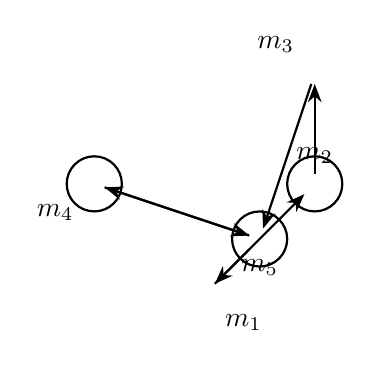
\begin{tikzpicture}[thick, scale=0.7]
    % Nodes with labels
    \node (n1) at (0, 0) [label=below right:$m_1$] {};
    \node (n2) at (2, 2) [label=above:$m_2$] {};
    \node (n3) at (2, 4) [label=above left:$m_3$] {};
    \node (n4) at (-2, 2) [label=below left:$m_4$] {};
    \node (n5) at (1, 1) [label=below:$m_5$] {};
    
    % Edges
    \draw[->, >=Stealth] (n1) edge (n2);
    \draw[->, >=Stealth] (n2) edge (n3);
    \draw[->, >=Stealth] (n3) edge (n5);
    \draw[->, >=Stealth] (n5) edge (n1);
    \draw[->, >=Stealth] (n4) edge (n5);
    \draw[->, >=Stealth] (n5) edge (n4);
    
    % Circle around m2
    \draw (n2) circle (0.5);
    
    % Circle around m4
    \draw (n4) circle (0.5);
    
    % Circle around m5
    \draw (n5) circle (0.5);
\end{tikzpicture}
\]

\end{document}